%%%%%%%%%%%%%%%%%%%%%
%								%
%	APENDICES					%
%								%
%%%%%%%%%%%%%%%%%%%%%

\appendix
\newpage

\chapter{Teoria de Grafos}\label{ap:apendice_graph_theory}
inicio de mi grafo \cite{book_introduction_graph_theory}
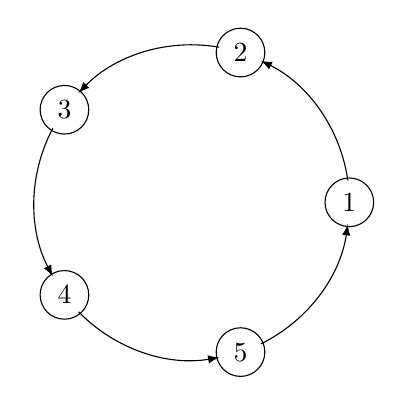
\begin{tikzpicture}

\def \n {5}
\def \radius {2cm}
\def \margin {8} % margin in angles, depends on the radius

\foreach \s in {1,...,\n}
{
test
  \node[draw, circle] at ({360/\n * (\s - 1)}:\radius) {$\s$};
  \draw[->, >=latex] ({360/\n * (\s - 1)+\margin}:\radius) 
    arc ({360/\n * (\s - 1)+\margin}:{360/\n * (\s)-\margin}:\radius);
}
\end{tikzpicture}

Final de mi grafo

\chapter{Catalog management handled with relational \dataBasesDB}\label{ap:apendice_ecommerce_catalog_relational}

\begin{figure}[h!]
	\centering
	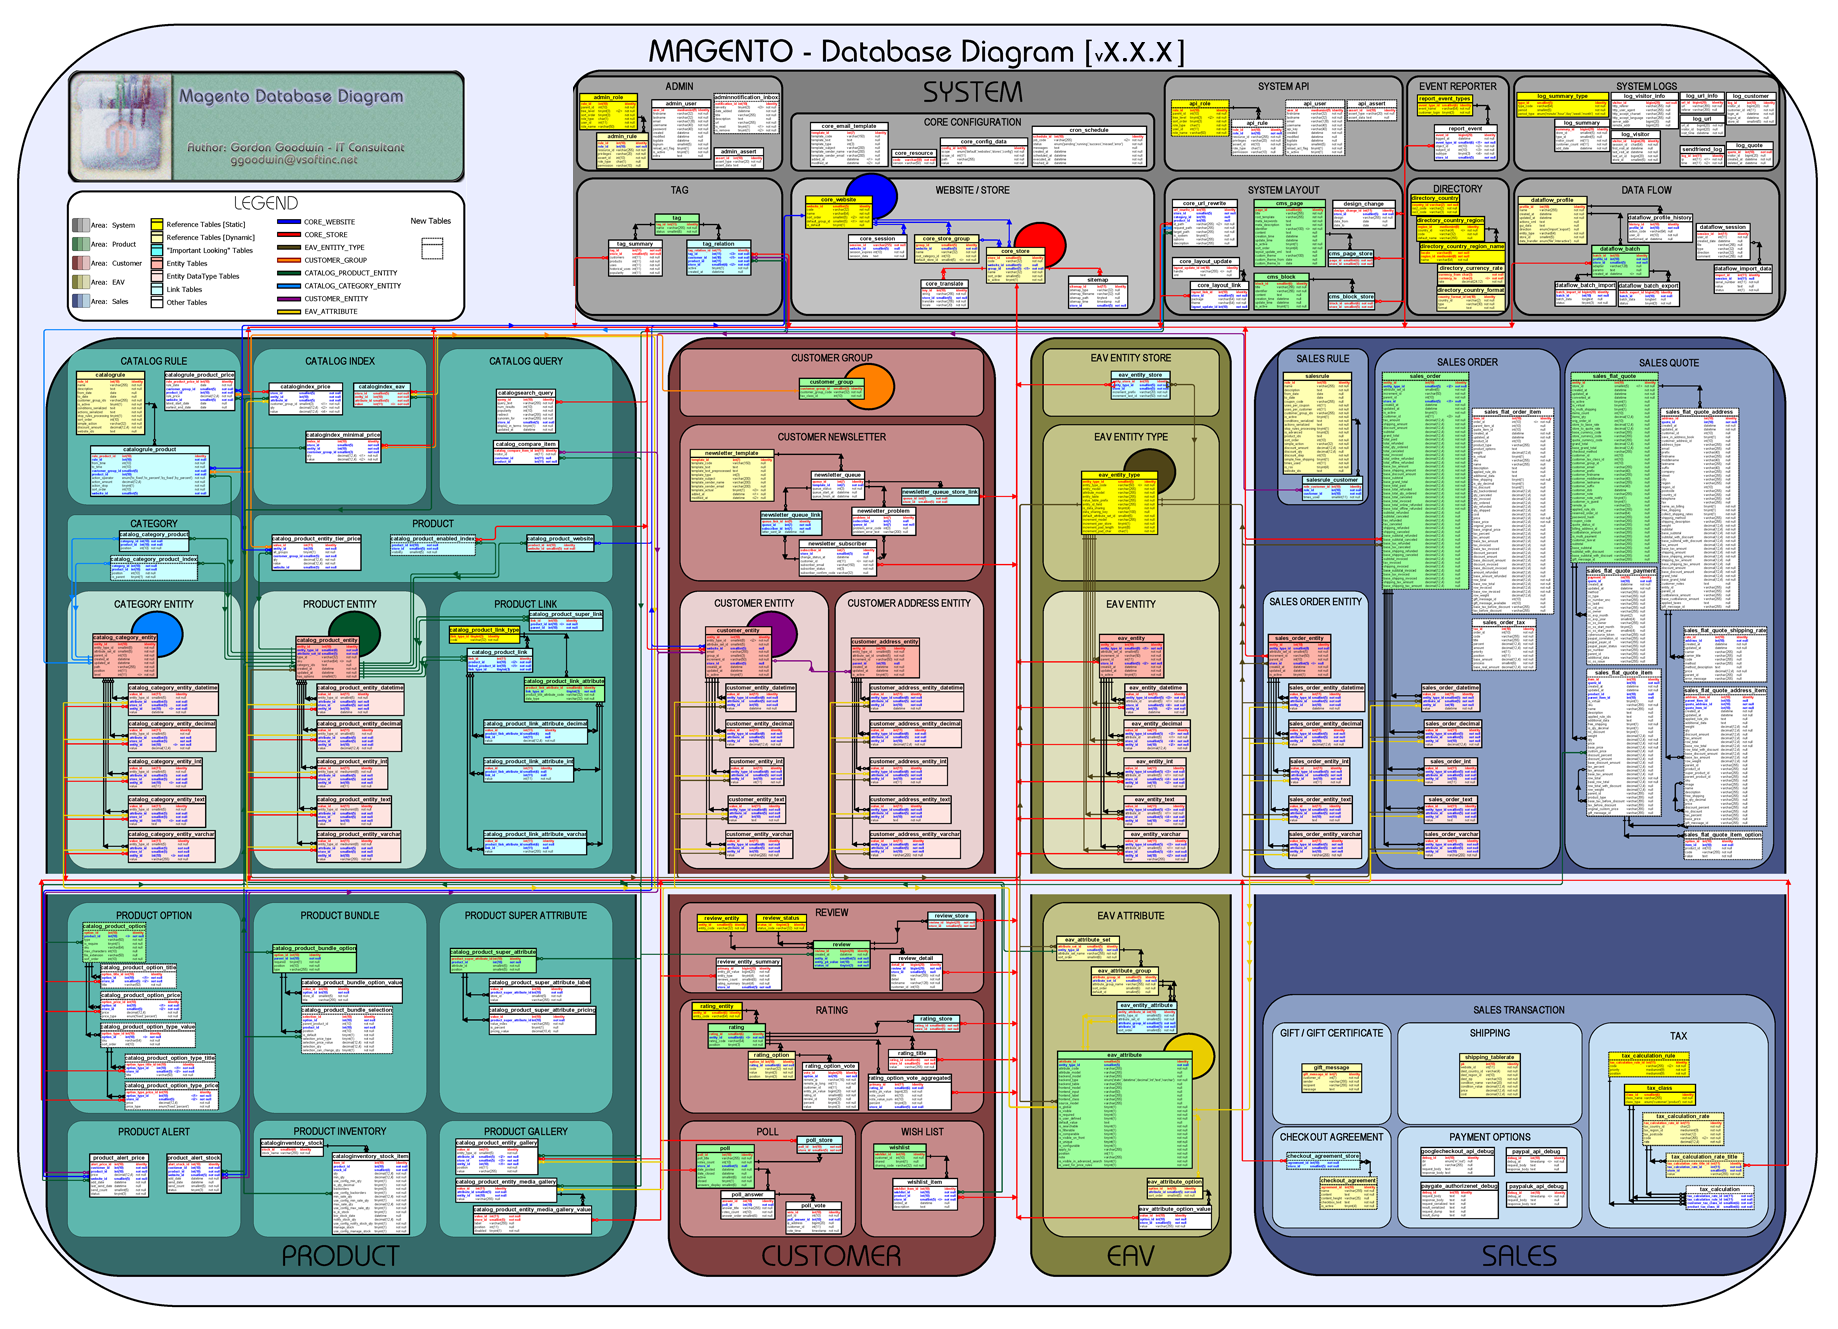
\includegraphics[width=0.8\textwidth]{figuras/apendice/magento_sample_database_diagram.png}
	\caption{\schemasDB de \nameMagento \ecommerce \frameworkPC.}
	\label{ap:figure:catalog_magento}
\end{figure}

\begin{figure}[h!]
	\centering
	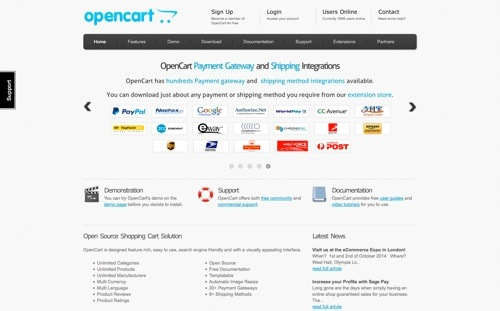
\includegraphics[width=0.5\textwidth]{figuras/apendice/openCartWebsite.jpg}
	\caption{\schemasDB de \ofBizNAME.}
	\label{ap:figure:catalog_ofbiz}
\end{figure}

\chapter{¿Qué es Hadoop? \cite{online_hadoop_description}}\label{ap:apendice_hadoop_description}
\apacheNAME \hadoopNAME es un proyecto software \openSourcePC que permite el procesamiento distribuido de gran cantidad de datos a través de \clustersAS de \serversAS. Esta diseñado para \scaleUpQA desde un único \serverAS a miles de máquinas, con un muy alto grado de tolerancia al fallo. En lugar de confiar en \highEndCPT \hardwarePC, la flexibilidad de estos \clustersAS proviene de la habilidad del \softwarePC en detectar y manejar fallos en la \applayer.

\subsubsection*{Arquitectura \highLevelCPT} 
\apacheNAME \hadoopNAME tiene dos pilares:

\begin{itemize}
	\item \hadoopYarnNAME asigna \cpuPC, memoria y almacenamiento para las aplicaciones corriendo en \clustersAS \hadoopNAME. La primera generación de \hadoopNAME podía correr solo aplicaciones \hadoopMapReduceNAME. \hadoopYarnNAME permite que otros entornos de aplicaciones (como \sparkNAME) para ejecutarse en \hadoopNAME, lo que abre un mundo de posibilidades.
	
	\item \hadoophdfsNAME es un sistema de archivos que se extiende por todos los nodos en su \clusterAS \hadoopNAME para almacenamiento de datos. Se conecta entre si a los sistemas de archivos en muchos nodos locales para convertirlos en un sistema de archivos grandes.
\end{itemize}

\hadoopNAME se complementa con un ecosistema de proyectos de \apacheNAME, como Pig\cite{online_ibm_meaning_pig}, Hive\cite{online_ibm_meaning_hive} y Zookeeper\cite{online_ibm_meaning_zookeeper}, para extender el valor de \hadoopNAME y mejorar su \usabilityQA.


\subsubsection*{Entonces, ¿Cuál es el problema?}

\hadoopNAME cambia la economía y la dinámica de la computación a gran escala. Su impacto puede reducirse a cuatro características sobresalientes.

\hadoopNAME permite una solución de computación que es:

\begin{itemize}
	\item \textbf{\scalableQA}- Nuevos nodos pueden ser agregados según sean necesarios, y agregados sin la necesidad de cambiar el formato de los datos, como los datos son cargados, como los \textit{jobs} son escritos, o las aplicaciones en la parte superior.
	
	\item \textbf{\costEffectiveCPT}- \hadoopNAME trae computación paralela masiva a las maquinas de los servidores. El resultado es una considerable disminución en los costos por \terabytePC de almacenamiento. lo cual hace asequible para modelar todos sus datos.
	
	\item \textbf{\flexibleQA}- \hadoopNAME no tiene esquema, y puede absorber cualquier tipo de datos, estructurados o no, desde cualquier numero de fuentes. Los datos de múltiples fuentes pueden ser unidos y se agregan arbitrariamente para permitir análisis que ningún otro sistema puede proporcionar.
	
	\item \textbf{\faultTolerantQA}- Cuando se pierde un nodo, el sistema redirige el trabajo a otra ubicación de los datos para seguir con el procesamiento sin perder el ritmo.
\end{itemize}

\chapter{Conexiones \stateful y \stateless }\label{ap:apendice_connection_statful_stateless}

Mantener el estado o ser \stateful significa que algunos dispositivos mantienen \trackCPT de otro dispositivo o una conexión, ya sea temporal o largo periodo de tiempo. Cuando se agrega el nombre de una persona en una libreta de direcciones y se observa su cumpleaños y teléfono, se podría decir que se esta manteniendo el estado de esa persona. En la \webINT una \cookieINT es un mecanismo \stateful que permite a los \webserverINT mantener \trackCPT de información de las personas, tal como se describe en un momento \cite{online_connection_stateful_stateless}.
%Keeping state or being stateful means that some device is keeping track of another device or a connection, either temporarily or over a long period of time. When I put someone's name in my address book and note their birthday and phone number, one could say that I am maintaining state for that person. On the Web, a cookie is a stateful mechanism that allows Web servers to keep track of information about people, as described in a moment.


Una conexión \stateful es una en la cual cierta información sobre una conexión entre dos sistemas es retenida para uso futuro. En algunos casos, la conexión es mantenida abierta incluso a través de dos sistemas que podrían no estar transmitiendo información(i.e., la conexión en si misma mantiene el estado)\cite{online_connection_stateful_stateless}.
%A stateful connection is one in which some information about a connection between two systems is retained for future use. In some cases, the connection is kept open even though the two systems might not be transmitting information (i.e., the connection itself retains state).

En contraste, una conexión \stateless es aquella en que no hay información retenida por el \senderINT ó \receiverINT. El \senderINT transmite un paquete al \receiverINT sin esperar ninguna confirmación de recepción. El \receiverINT recibe el paquete sin ninguna configuración de la conexión anterior  \cite{online_connection_stateful_stateless}.
%In contrast, a stateless connection is one in which no information is retained by either sender or receiver. The sender transmits a packet to the receiver and does not expect an acknowledgment of receipt. The recipient receives the packet without any prior connection setup.


		